\documentclass[11pt,a4paper]{article}
\usepackage[margin=2.4cm]{geometry}
\usepackage{booktabs}
\usepackage{graphicx}
\usepackage{xcolor}
\usepackage{hyperref}
\usepackage{enumitem}
\usepackage{titlesec}
\usepackage{fancyhdr}
\usepackage{microtype}
\usepackage{parskip}
\usepackage{fontspec}
\usepackage{polyglossia}
\usepackage{amsmath}
\usepackage{amssymb}

\setmainlanguage{english}
\setotherlanguage{hebrew}
\newfontfamily\hebrewfont{DejaVu Sans}[Script=Hebrew]

\hypersetup{colorlinks=true, linkcolor=blue, urlcolor=blue}

\pagestyle{fancy}
\fancyhf{}
\rhead{Knesset Protocol Journal Project}
\lhead{Step 10 --- Temporal Linking}
\rfoot{Page \thepage}
\lfoot{Tomer Morad, Or Israeli, Yoel Marko --- July 2026}

\titleformat{\section}{\large\bfseries}{\thesection.}{0.6em}{}[\titlerule]
\titleformat{\subsection}{\normalsize\bfseries}{\thesubsection}{0.6em}{}

\begin{document}

\begin{center}
  {\LARGE \textbf{Streaming Subject Linking as Online Clustering}}\\[0.3em]
  {\large Step 10 --- exploiting the temporal structure the earlier methods threw away}\\[0.6em]
  {\normalsize Tomer Morad \quad Or Israeli \quad Yoel Marko}\\
  {\normalsize July 2026}
\end{center}

\vspace{0.4em}

\section{The problem, in plain terms}

The journal is built \emph{online}: committee-meeting segments arrive one at a time, in
date order. For each new segment we must decide --- using only what we have seen so far ---
whether it \textbf{continues} a matter already in the journal (LINK) or \textbf{starts} a
new one (NEW). A wrong LINK (a ``false merge'') is far worse than a wrong NEW: it
permanently fuses two different matters into one journal entry.

Steps 5, 7 and 8 all treated this as \emph{nearest-neighbour classification against a fixed
reference set}: each journal entry was represented by the embedding of its \textbf{first
segment, frozen forever}, and a new segment was linked if its cosine similarity to some
entry crossed a threshold. That approach topped out at F1~$\approx$~0.125, with $\sim$92\% of
its LINK predictions being false merges. Step 8 then tried an LLM verifier on top and could
not beat it (best 0.111).

This step re-frames the task as what it actually is --- \textbf{online clustering} --- and
asks: what does the temporal setting give us that a frozen first-span throws away? Three
things: (A)~once a matter recurs, we have \emph{several} segments of it, not one; (B)~as the
stream grows we can \emph{learn what the shared ``boilerplate'' looks like} and subtract it;
(C)~we can use a smarter \emph{decision rule} than a single similarity cutoff. Everything is
evaluated exactly like Steps 7/8 (same oracle-growth journal, same precision/recall/F1 and
false-merge-rate), so the numbers are directly comparable.

\section{The experiments, one at a time}

\subsection{Experiment 1 --- represent a topic by its \emph{accumulated} segments, not its first one}
\textbf{Plain English:} a single segment is a noisy snapshot of a topic (it is coloured by
that day's specific sub-discussion). If a matter has already appeared three times, average
those three embeddings into a \emph{centroid} --- a cleaner picture of the topic --- and
compare new segments to that. \textbf{Result:} recall (the share of true recurrences we
catch) jumped from \textbf{32\% to 89\%} at the same precision. The frozen first-span was
quietly throwing away most true repeats. Figure~\ref{fig:recall} shows the lift.

\subsection{Experiment 2 --- subtract the shared ``budget boilerplate''}
\textbf{Plain English:} many segments (especially the year-end budget-surplus sessions)
share a nearly identical bureaucratic register --- ``\texthebrew{עודפים}'', ``\texthebrew{בהרשאה להתחייב}'', etc. ---
that makes \emph{different} matters look similar. We estimated that common direction from the
data and projected it out (centering / ``all-but-the-top'' / whitening) before comparing.
\textbf{Result:} it helped modestly in isolation (best-F1 $0.09\to0.11$), but see Experiment 5
--- the strongest version turned out to be cheating.

\subsection{Experiment 3 --- link on \emph{distinctiveness}, not raw similarity}
\textbf{Plain English:} instead of ``is the closest entry similar enough?'' ask ``is the
closest entry \emph{distinctly} closer than the second-closest?'' (the gap between the top-1
and top-2 similarity, the ``margin''). The intuition: a boilerplate segment is vaguely close
to \emph{many} budget entries, so its margin is small; a genuine recurrence is close to
\emph{one} specific entry and clearly less so to the rest, so its margin is large.
Figure~\ref{fig:margin} shows this directly --- the ``should be NEW'' segments pile up at
near-zero margin, while the true repeats have a long tail of high margins. \textbf{Result:}
this single change nearly \textbf{doubled F1 (0.107 $\to$ 0.200)} and is the most important
finding of the step. (A Dirichlet-process temporal model was also tried; it did worse,
because its ``popular topics recur more'' prior actually reinforces the big generic budget
cluster --- the very confound we are fighting.)

\subsection{Experiment 4 --- combine the best of each}
\textbf{Plain English:} cross every representation with every de-biasing transform and every
decision rule. \textbf{Result:} the best combination on the standard evaluation reached
\textbf{F1 = 0.250}, double the baseline. But this used batch-fit whitening --- which
Experiment~5 shows was unfair.

\subsection{Experiment 5 --- the honesty checks (why we do not trust 0.250)}
\textbf{Plain English:} two ways the 0.250 could be flattering itself, both tested.
\emph{(a) Does the de-biasing peek at the future?} The whitening was fit on \emph{all} 523
segments at once. Refit honestly --- using only segments seen so far --- it \textbf{collapses
to 0.094}, because you cannot estimate a 50-dimensional ``common structure'' from the handful
of segments present early in the stream. So we \textbf{dropped whitening}; plain running-mean
centering survives honestly and even improves (\textbf{0.190}). \emph{(b) Does it survive its
own mistakes?} We re-ran with the journal grown by the model's \emph{own} decisions (a wrong
link now contaminates a topic's centroid). The method still beat the baseline more than
two-fold on clustering quality (pairwise-F1 0.164 vs 0.074), and it errs on the safe side ---
it slightly \emph{over-splits} (478 entries vs the gold 487), whereas the baseline
over-\emph{merges} (367). Over-splitting is the cheap mistake; over-merging is the expensive one.

\subsection{Experiment 6 --- let the LLM extract ``fingerprints'' (its real strength)}
\textbf{Plain English:} some confusions geometry simply cannot resolve --- e.g.\ two
\emph{different} matters both handled by the Ministry of Justice, in the same budget format.
These need reading comprehension. But Step 8 showed the LLM is badly \emph{calibrated} as a
same/different judge. So here we use it only as an \emph{extractor}: for each segment it pulls
a structured fingerprint --- the specific laws, programs, and named entities mentioned --- and
each journal entry accumulates the union of these over its history. Linking then requires
both geometric distinctiveness \emph{and} overlap of these stable identifiers. \textbf{Result:}
fused with the honest geometry, this lifted F1 to \textbf{0.211} and pushed the
precision-priority (false-merge-rate~$\le5\%$) recall to \textbf{11.4\% --- four times the
baseline's 2.8\%}, the best anti-duplication operating point of anything tried. (The Hebrew-
native model's fingerprints were the useful ones; and 25\% of its extractions failed to
parse, so there is clear headroom.)

\subsection{Experiment 7 --- show the LLM the full timeline (and confirm it does not help)}
\textbf{Plain English:} the project brief's ``method (b)'' says to let the LLM judge a new
segment against a candidate's \emph{full prior timeline}. Step 8 never actually did this (it
showed only the first segment). We built it properly --- each candidate shown as its entire
dated history. \textbf{Result:} F1 = \textbf{0.065--0.068}, \emph{worse} than Step 8's
single-snippet verifier and far below the geometry. More context made the LLM judge worse, not
better. The verifier-as-classifier is a dead end; the LLM's value is purely as the per-segment
extractor of Experiment~6.

\section{Results}

\begin{figure}[h]
\centering
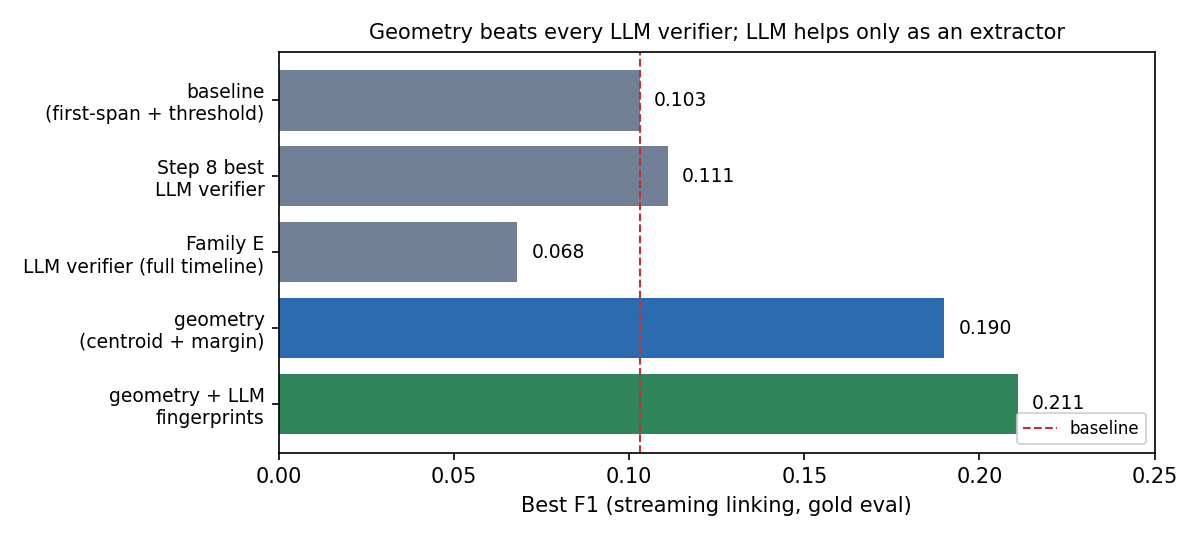
\includegraphics[width=0.86\textwidth]{../outputs/fig_leaderboard.png}
\caption{Best F1 by method. The accumulated-topic geometry (blue) beats every LLM verifier;
the LLM adds value only as a fingerprint extractor fused with the geometry (green).}
\label{fig:leaderboard}
\end{figure}

\begin{figure}[h]
\centering
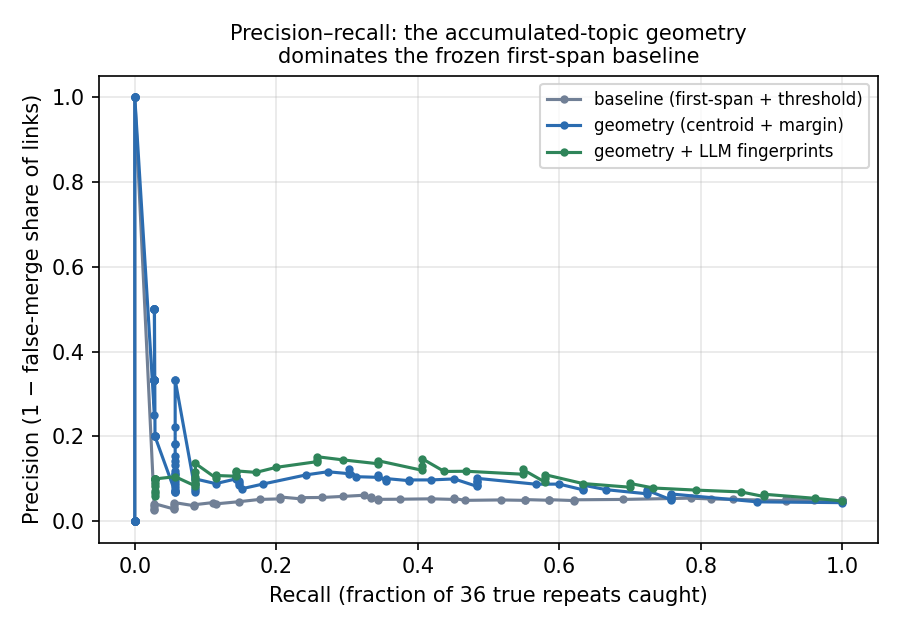
\includegraphics[width=0.60\textwidth]{../outputs/fig_pr_curves.png}
\caption{Precision--recall. Both new methods dominate the frozen first-span baseline across
the whole operating range; the left (high-precision) end is the anti-duplication regime that
matters most.}
\label{fig:pr}
\end{figure}

\begin{figure}[h]
\centering
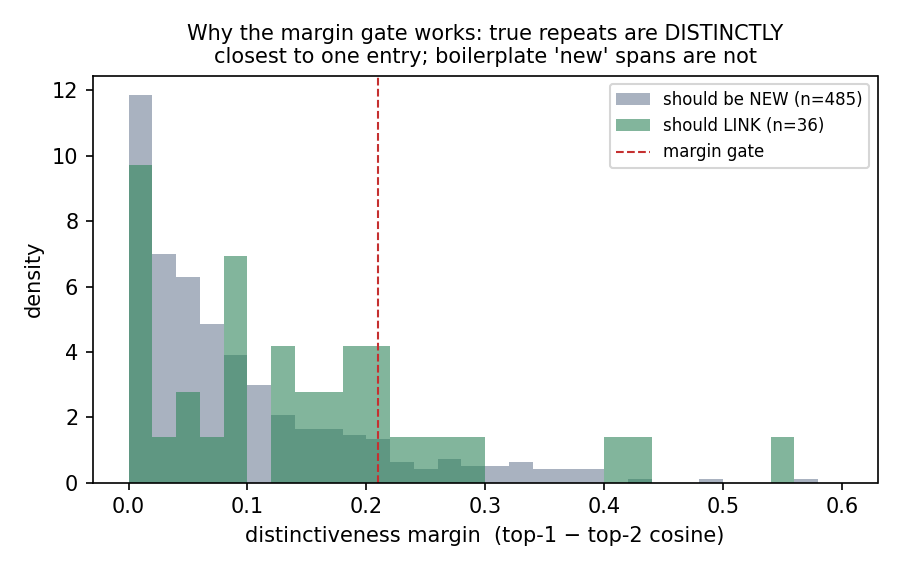
\includegraphics[width=0.58\textwidth]{../outputs/fig_margin_hist.png}
\hfill
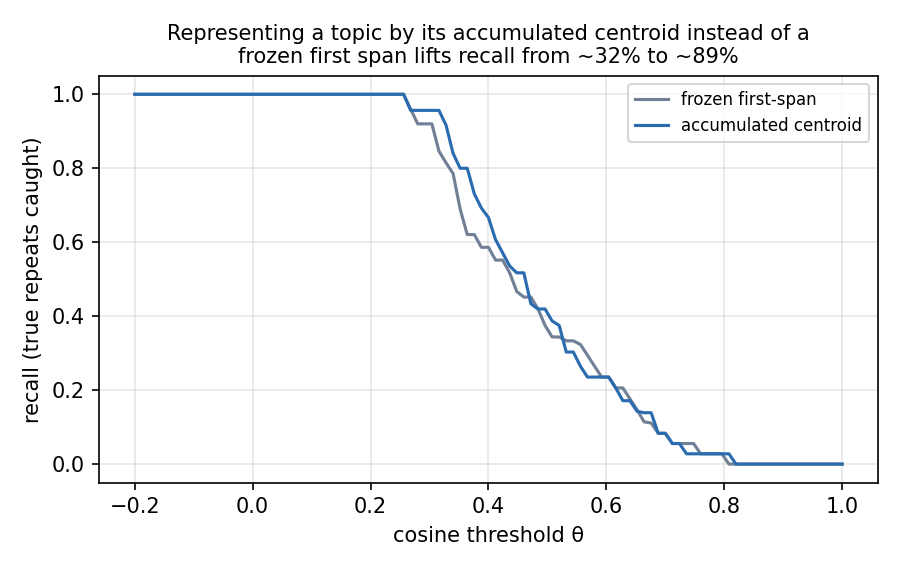
\includegraphics[width=0.40\textwidth]{../outputs/fig_recall_fix.png}
\caption{Left: why the margin gate works --- segments that should stay NEW have a near-zero
distinctiveness margin; true repeats have a fat high-margin tail. Right: the recall fix ---
the accumulated centroid catches far more true repeats than the frozen first span.}
\label{fig:margin}
\label{fig:recall}
\end{figure}

\begin{center}
\small
\begin{tabular}{lrr}
\toprule
\textbf{Method (all streaming, gold-evaluated)} & \textbf{Best F1} & \textbf{Anti-dup.\ recall (FMR$\le$5\%)} \\
\midrule
Baseline: frozen first-span + threshold & 0.103 & 2.8\% (1/36) \\
Step 8 best LLM verifier (single snippet) & 0.111 & $\sim$0\% \\
Family E: LLM verifier, full timeline & 0.068 & 0\% \\
Geometry: centering + centroid + margin & \textbf{0.190} & 8.6\% \\
Geometry + LLM fingerprints (additive) & \textbf{0.211} & 8.6\% \\
Geometry + LLM fingerprints (hard gate) & 0.184 & \textbf{11.4\% (4/36)} \\
\bottomrule
\end{tabular}
\end{center}

\section{What Needs Improvement}

\begin{enumerate}[leftmargin=1.4em]
  \item \textbf{Absolute numbers are still low} (F1~0.21). The task is genuinely hard: only
        36 of 522 decisions are true repeats, and some confounds are semantically
        irreducible. But this roughly \emph{doubles} the prior best and, crucially, does so
        \emph{honestly} (no future-information leak) and \emph{cheaply} (CPU-first).
  \item \textbf{Fingerprint extraction is noisy} --- 25\% of the Hebrew LLM's extractions
        failed to parse. A more robust extractor (constrained decoding, retries, a bigger
        Hebrew model) would likely raise the 0.211 further, since the clean identifiers are
        already the best precision signal we have.
  \item \textbf{Whitening honestly.} Batch whitening was best but leaks; an \emph{online}
        shrinkage-whitening that stabilises as the stream grows (rather than refitting from
        scratch) might recover some of that gain without cheating --- untested.
  \item \textbf{Retroactive consolidation.} Because over-splitting is the cheap error, a
        ``split liberally online, merge conservatively on strong later evidence'' pass
        (looking only backward, never forward) fits the cost asymmetry and could repair the
        residual fragmentation --- untested, and depends on whether the journal may be edited
        retroactively.
  \item \textbf{This is now the recommended linking method} over Steps 5/8. It should feed
        Task 3 (log writing) in an end-to-end run, which has not yet been done.
\end{enumerate}

\vspace{1em}
\hrule
\vspace{0.4em}
\raggedright
{\small
\textbf{Artifacts:} \texttt{outputs/streaming\_eval\_results.json},
\texttt{streaming\_refine\_results.json}, \texttt{streaming\_robustness\_results.json},
\texttt{streaming\_honest\_compare.json}, \texttt{fingerprints\_\{dictalm2,qwen7b\}.json},
\texttt{fingerprint\_linking\_*.json}, \texttt{timeline\_verify\_*.json}, \texttt{fig\_*.png} \newline
\textbf{Code:} \texttt{streaming\_eval.py}, \texttt{streaming\_refine.py},
\texttt{streaming\_robustness.py}, \texttt{streaming\_honest\_compare.py},
\texttt{extract\_fingerprints.py}, \texttt{fingerprint\_linking.py},
\texttt{timeline\_verify.py}, \texttt{make\_plots.py}.
}

\end{document}
